\documentclass [12pt] {oblivoir}

\usepackage{fapapersize}
\usefapapersize{210mm,297mm,20mm,*,20mm,22mm}

\setlength\parindent{0pt}

\usepackage{graphicx}
\usepackage{mathtools}
\usepackage{amsmath}
\usepackage{upgreek}

\begin{document}
원형의 파이프 $N$개가 있다.

각 파이프의 반지름을 안다고 하자. 파이프를 모두 같은 방향으로 놓으려고 한다.

즉, 파이프는 원으로 생각할 수 있다. 또, 모든 파이프는 바닥에 닿아 있어야 한다.

즉, 어떤 파이프든지 다른 파이프 위에 있어서 바닥과 떨어져 있으면 안된다.

파이프가 원으로 보이는 방향에서 보았을 때 놓았을 때 왼쪽 끝부터 오른쪽 끝까지의 거리를 가능한 최소화하라.

아래 그림은 5개의 파이프를 배치한 두가지 방법을 보여준다.

왼쪽 방법보다 오른쪽 방법의 왼쪽 끝에서 오른쪽 끝까지의 거리가 더 작음을 알 수 있다.

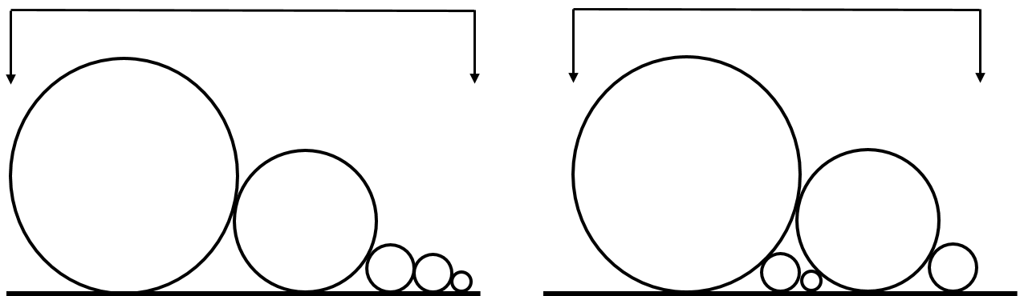
\includegraphics[scale=0.5]{n4.png}


이 문제는 주최측이 계산한 답에 대한 비례로 점수가 주어진다. 아래 채점 방식을 확인하라.

- 제한시간: 전체 테스트 케이스는 30개 이하이며, 전체 수행 시간은 2초 이내. (Java 4초 이내)

제한 시간을 초과하면 제출한 소스코드의 프로그램이 즉시 종료되며, 그때까지 수행한 결과에서 테스트 케이스를 1개 그룹 이상 통과하였더라도 점수는 0점이 됩니다.
그러나, 제한 시간을 초과하더라도 테스트 케이스를 1개 그룹 이상 통과하였다면 '부분 점수(0 $<$ 점수 $<$ 만점)'를 받을 수 있으며, 이를 위해서는, C / C++ 에서 "printf 함수" 사용할 경우, 프로그램 시작부분에서 "setbuf(stdout, NULL);"를 한번만 사용하십시오.
C++에서는 "setbuf(stdout, NULL);"와 "printf 함수" 대신 "cout"를 사용하고, Java에서는 "System.out.printIn"을 사용하시면, 제한 시간을 초과하더라도 '부분 점수'를 받을 수 있습니다.

※ 언어별 기본 제공 소스코드 내용 참고

만약, 제한 시간을 초과하지 않았는데도 '부분 점수'를 받았다면, 일부 테스트 케이스를 통과하지 못한 경우 입니다.

- 메모리 사용 제한 : heap, global, static 총계 256MB, stack 100MB

- 제출 제한 : 최대 10회 (제출 횟수를 반영하여 순위 결정)


메모리 사용 제한

heap, global, static (총계) : 256MB

stack : 100MB

입력

입력 파일에는 여러 테스트 케이스가 포함될 수 있다.

파일의 첫째 줄에 테스트 케이스의 개수를 나타내는 자연수 T가 주어지고,
이후 차례로 $T$ 개의 테스트 케이스가 주어진다. $(1 \le T \le 30 )$
각 테스트 케이스의 첫 줄에는 파이프의 개수 $N$ 이 주어진다. $(3 \le N \le 100 )$
다음 줄에 각 파이프의 반지름이 $N$ 개의 정수로 주어진다.
반지름은 1 이상 1,000,000 이하이다.

- 점수 : 최대 10회 제출하여 취득한 각각의 점수 중에서 최대 점수 (만점 200점)
각 테스트 케이스에 대해 주최측이 계산한 답과 비교하여 산정된 점수를 테스트케이스 모두에 대해 평균한다. 전체 평균이 200점을 넘을 수도 있다.
이 때는 점수가 200점으로 결정된다.

 ㆍ 참가자가 제출한 해에서 원이 겹치는 등 문제의 조건을 위배하면 0점이다.

 ㆍ 그 이외의 경우, 주최측이 계산한 왼쪽 끝 오른쪽 끝 거리가 $A$, 제출된 거리가 $B$ 일때, 아래 식에 따라 점수가 정해진다.

    -  $B \le 2A$ 인 경우: $200(2 - BA)$ 점

    -  $B > 2A$ 인 경우: $0$ 점

출력

각 테스트 케이스의 답을 순서대로 표준출력으로 출력하여야 하며,

각 테스트 케이스마다 첫 줄에는 “Case \#C”를 출력하여야 한다. 이때 C는 테스트 케이스의 번호이다.

다음 $N$개의 줄에, 입력에 주어진 순서대로의 각 파이프 중심의 $x$ 좌표를 출력한다.
파이프들의 위치는 어디이든 상관없으나 모든 좌표 값의 절대값이 1018 이하라야 한다.
좌표 값은 실수로 적어도 소수점 이하 10자리까지 출력해야 정확한 채점을 보장할 수 있다.
출력한 원들의 위치에 대해, 임의의 두 원을 잡았을 때 (중심사이의거리) $\ge$ (반지름의길이합) - 10 - 6을 만족해야 점수가 주어진다.

입출력예

입력

2

5

290328 356166 438877 410830 219438

7

405391 510242 439253 547312 465626 534027 608087

출력

Case \#1

1334579.04753950797021389008

2790350.17604429880157113075

620665.09850643284153193235

2025304.61457753228023648262

0.00000000000000000000

Case \#2

0.00000000000000000000

6058220.07462551258504390717

2026643.68445300729945302010

3007272.94760193023830652237

4016911.88764336891472339630

5014221.98165024258196353912

993001.50456482195295393467

\end{document}
